\chapter[Modelo de extracción paralelizado]{
    Modelo de extracción paralelizado
}
\label{chapter:parallel}

Como respuesta a las limitaciones identificadas en \gls{feets}, decidimos desarrollar una nueva versión de la herramienta que aborde estas problemáticas. El objetivo principal de esta nueva versión, y la mayor motivación que impulsó a hacer este trabajo, fue mitigar el cuello de botella producido por la ejecución secuencial de los extractores de características, optando por un algoritmo paralelizado que haga un mejor uso de los recursos del sistema.

En este capítulo explicaremos cómo se llevó a cabo la implementación de este nuevo modelo de extracción paralelizado. Hablaremos en detalle sobre la problemática que intentamos resolver con este modelo, las inconveniencias que surgieron al buscar una solución al problema y también sobre las decisiones de diseño que nos parecieron relevantes durante el proceso de desarrollo.

\section{El algoritmo secuencial}

Como se explica en el \autoref{chapter:feets}, la versión original de \gls{feets} ejecuta los extractores seleccionados de manera secuencial, es decir, procesando uno a la vez. No obstante, dado que la aplicación está diseñada para el manejo de extensos volúmenes de datos, es esperable que algunas de las características requieran un tiempo prolongado de procesamiento. Con esto en mente, buscamos optimizar el uso de los recursos del sistema para que se enfoquen en el proceso de extracción y que no se desaprovechen en tareas secundarias.

El principal problema de la ejecución secuencial, entonces, es que introduce una capa adicional a la complejidad temporal del programa, haciendo que el tiempo total de procesamiento no solo dependa del costo individual de cada extractor, sino que además crezca linealmente con la cantidad de extractores seleccionados. Como resultado, el algoritmo secuencial hace que los tiempos de ejecución de \gls{feets} sean innecesariamente largos, limitando la eficiencia y el uso práctico de la aplicación cuando se quieren extraer múltiples características.

\section{Un primer acercamiento paralelizado}

Las demoras ocasionadas por el algoritmo secuencial pueden ser solventadas siguiendo un esquema paralelizado, que sea capaz de ejecutar más de un extractor a la vez. Siguiendo este acercamiento, una primera solución \emph{naive} podría ser ejecutar todos los extractores seleccionados en simultáneo, procesando todas las características necesarias en un mismo espacio de tiempo en lugar de hacerlo en orden secuencial.

A primera vista, el método \emph{naive} parece ser justo lo que buscamos, porque elimina por completo el impacto que tiene la cantidad de extractores seleccionados sobre el tiempo total del proceso de extracción. En realidad, el algoritmo presenta un problema fundamental, y es que parte de la suposición de que todos los extractores son independientes entre sí cuando en la práctica puede suceder que un extractor dependa de la extracción previa de otras características.

\section{El problema de las dependencias}

En \gls{feets}, un extractor con dependencias es aquel que, además de los vectores proporcionados por la serie temporal, requiere de la entrada de una o más características que deben ser calculadas previamente por otros extractores. Estos requerimientos imponen una restricción sobre el orden en que deben ejecutarse los extractores para el correcto funcionamiento del programa, pues un extractor no debería comenzar su ejecución a menos que todas sus dependencias hayan sido satisfechas.

El extractor \texttt{Sig\-na\-ture}, por ejemplo, depende de las características \texttt{Pe\-riod\-LS} (período) y \texttt{Am\-pli\-tude} (amplitud) para computar \texttt{SignaturePhMag}, un histograma bidimensional de una \acrfull{lc} en el espacio fase-magnitud. Estas características son calculadas por los extractores \texttt{LombScargle} y \texttt{Amplitude} respectivamente, cuya ejecución debe venir antes que la de \texttt{Signature} si queremos asegurar que sus dependencias estén disponibles para ese momento.

El problema de la solución \emph{naive} es que computa todas las características al mismo tiempo, por lo que naturalmente se rompe al introducir dependencias en el asunto: es imposible que las dependencias de un extractor estén disponibles al momento de su ejecución si al mismo tiempo también se están ejecutando los extractores que las computan. Si bien el algoritmo optimiza los tiempos de procesamiento, no presenta ninguna noción de orden, por lo que funciona correctamente siempre y cuando los extractores presentes no tengan dependencias de características.

Por el otro lado, pese al mal desempeño que tiene la versión secuencial de \gls{feets}, su capacidad de ejecutar los extractores en orden le da una ventaja que la solución \emph{naive} no posee: puede asegurar el orden correcto de las dependencias. Para esto, la versión secuencial se encarga de ordenar el proceso de extracción mediante lo que llamamos como un ``plan de ejecución'', una lista que comprende tanto a los extractores seleccionados por el usuario como a los extractores que se necesitan para cumplir con todas sus dependencias. El plan de ejecución está ordenado de forma tal que cada extractor aparece estrictamente después de los extractores de los que depende, por lo que el algoritmo secuencial simplemente debe encargarse de ejecutar los extractores en el orden establecido y de esta forma garantiza que cuando tenga lugar la extracción de una característica, todas sus dependencias hayan sido ya computadas.

El desafío central, entonces, radica en proporcionar un esquema de ejecución inteligente que equilibre los aspectos positivos de las dos soluciones propuestas. Por un lado, queremos maximizar el cómputo paralelizado para reducir los tiempos de ejecución de manera similar al método \emph{naive}, pero también queremos que el algoritmo sea capaz de lidiar con las dependencias entre los distintos extractores, como lo hace la versión secuencial.

\section{Nuestra solución}

Para la nueva versión de \gls{feets}, hemos desarrollado un esquema que logra cumplir con los objetivos propuestos, solucionando así los problemas de desempeño obtenidos con la versión original de la herramienta y asegurando la correcta resolución de dependencias.

La idea detrás del algoritmo es la de ejecutar en paralelo la mayor cantidad de extractores posibles, dejando en espera aquellos que dependan de características aún no computadas. A medida que los primeros extractores se terminen de ejecutar, se irán liberando del estado de espera aquellos extractores que dependan de sus características, quienes pasarán a correr en paralelo junto a los demás extractores en ejecución. A su vez, cuando estos nuevos extractores finalicen, se iniciarán los extractores que dependan de estos, repitiendo así el proceso sucesivamente hasta haber ejecutado todos los extractores.

En esta nueva versión, el proceso de extracción está modelado en la forma de un grafo dirigido al cual denominamos ``grafo de ejecución''. En esta estructura, cada nodo representa la ejecución de un extractor individual, y las aristas indican las relaciones de dependencia entre los distintos extractores. Cada nodo tiene que esperar a que sus vecinos entrantes hayan terminado su funcionamiento para poder iniciar, por lo que si dos nodos están en ramas distintas es porque son independientes entre sí, y se pueden ejecutar en paralelo. Con este modelo, el algoritmo inicia con la ejecución paralela de todos los nodos ``huérfanos'' (sin dependencias), y continúa con la computación de los nodos que salen desde sus aristas; luego, se repite el mismo proceso partiendo desde estos nodos, y así sucesivamente con todos los que les siguen hasta haber procesado la totalidad del grafo.

\begin{figure}[!ht]
\centering
\begin{subfigure}{0.4\textwidth}
    \centering
    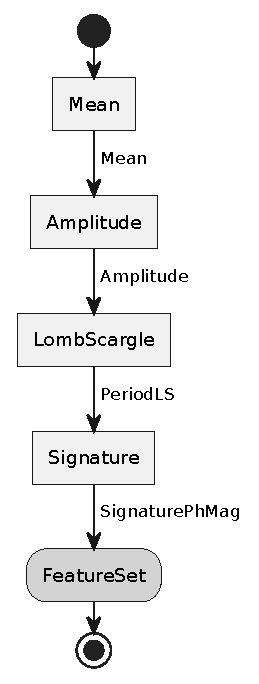
\includegraphics[width=.7\linewidth]{06_parallel/figures/sequential_ext.pdf}
    \caption{Plan de ejecución secuencial.}
\end{subfigure}%
\begin{subfigure}{0.6\textwidth}
    \centering
    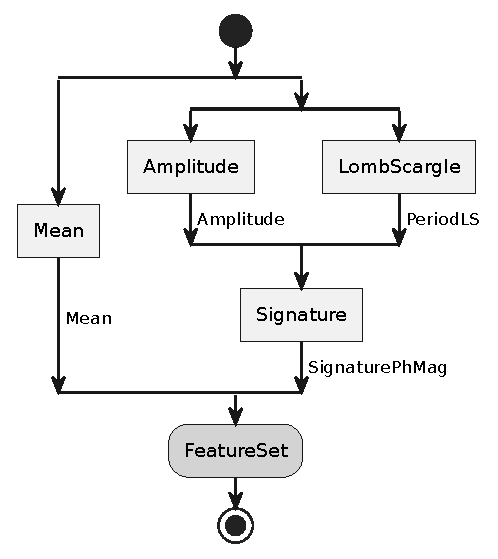
\includegraphics[width=.9\linewidth]{06_parallel/figures/parallel_ext.pdf}
    \caption{Grafo de ejecución paralelizado.}
\end{subfigure}

\caption{
    Esquema de ejecución de la extracción de características \texttt{Mean} y \texttt{SignaturePhMag} para el modelo secuencial y la nueva versión paralelizada. Las cajas representan los extractores individuales y las flechas indican el orden de ejecución. Una flecha que se divide en dos caminos distintos representa la paralelización de tareas, y las etiquetas en las flechas indican las características obtenidas por los extractores. Al final del proceso, se juntan todas las características extraídas en un \texttt{FeatureSet}, que se devuelve como salida.
}
\label{fig:execution_plans}
\end{figure}

La \autoref{fig:execution_plans} ilustra, a modo comparativo, el modelo secuencial de la versión original de \gls{feets} y el esquema paralelizado que implementamos en la nueva versión. Ambos modelos están aplicados al ejemplo de la extracción de \texttt{SignaturePhMag}, incorporando además la característica \texttt{Mean} a la selección, que no depende y no es dependencia de ninguna otra característica. En el enfoque secuencial, se observa que el plan de ejecución sigue una estructura con forma de cadena, ejecutando un solo extractor a la vez. En contraste, en el modelo paralelizado, se pueden identificar nodos independientes entre sí que se ejecutan en simultáneo, pero se conserva el orden de las dependencias cuando es necesario.

\section{Decisiones de diseño}

El ecosistema de Python ofrece diversas herramientas para la paralelización de tareas, pero para los propósitos de este proyecto optamos por el uso de la biblioteca \emph{Dask}\footnote{\url{https://www.dask.org/}} que se especializa en la ejecución de tareas distribuidas \citep{rocklin2015dask}. Entre los motivos detrás de esta elección se encuentran su facilidad de uso y su extensa documentación, pero también el hecho de que \emph{Dask} proporciona una \gls{api} robusta que permite modelar grafos de tareas para su ejecución en paralelo. Esta última funcionalidad es relevante porque funcionó como la base sobre la cual implementamos el grafo de ejecución utilizado en el nuevo modelo paralelizado de la extracción de características.

\emph{Dask} tiene también la ventaja de contar con distintos \emph{schedulers} internos que permiten decidir cómo se distribuyen las tareas según el \emph{hardware} disponible y la naturaleza del problema. De estos, nos interesan particularmente tres \emph{schedulers}:

\begin{itemize}
    \item \textbf{\texttt{synchronous}}. Ejecución secuencial, sin paralelismo.
    \item \textbf{\texttt{threads}}. Ejecución concurrente con \emph{multithreading}.
    \item \textbf{\texttt{processes}}. Ejecución paralelizada con \emph{multitprocessing}.
\end{itemize}

Todas las funcionalidades destinadas a la ejecución distribuida del modelo paralelizado las agrupamos en un nuevo módulo del sistema: \texttt{runner}. El módulo abstrae la comunicación con \emph{Dask}, definiendo una interfaz fija que proporciona los métodos necesarios para llevar a cabo la extracción paralelizada de características sin exponer el cómo se delegan las tareas a esta biblioteca.

La ventaja de tener el módulo \texttt{runner} con una interfaz fija es que, si al día de mañana se quiere reemplazar \emph{Dask} por otra biblioteca de ejecución distribuida, entonces solo hace falta reimplementar los métodos internos del módulo para que se comuniquen correctamente con este nuevo \emph{back end}. Estos cambios no deberían afectar el comportamiento externo de \texttt{runner}, lo que evita tener que hacer modificaciones en el resto del código, y además permite la ejecución de \emph{tests} automatizados para asegurar que el módulo funcione correctamente.